\documentclass[12pt, a4paper]{article}
\usepackage[utf8]{inputenc}
\usepackage[spanish]{babel}
\usepackage{graphicx}
\usepackage{tcolorbox}
\tcbuselibrary{listings, skins, breakable}
\usepackage{xcolor}
\usepackage{geometry}
\usepackage{tikz}
\usepackage{struktex}
\geometry{a4paper, margin=2cm, top=2.5cm, bottom=2.5cm}
\usepackage{hyperref}
\usepackage{setspace}

\definecolor{macred}{HTML}{FF5F56}
\definecolor{macorange}{HTML}{FFBD2E}
\definecolor{macgreen}{HTML}{27C93F}
\definecolor{landingB}{HTML}{006633} % Verde ESPE
\definecolor{landingC}{HTML}{0078D7} % Azul
\definecolor{accent}{HTML}{FFBD2E} % Naranja acento

\newtcblisting{maccode}[2][]{
  enhanced,
  colback=white,
  colframe=black!15,
  arc=8pt,
  boxrule=1pt,
  drop shadow=black!10,
  title={\textcolor{macred}{\Huge $\cdot$} \textcolor{macorange}{\Huge $\cdot$} \textcolor{macgreen}{\Huge $\cdot$} \hspace{0.5cm} \textcolor{black}{\textsf{\textbf{#2}}}},
  coltitle=black,
  fonttitle=\bfseries,
  listing only,
  listing options={
    language=Java,
    basicstyle=\ttfamily\scriptsize\color{black},
    keywordstyle=\color{blue}\bfseries,
    stringstyle=\color{green!50!black},
    commentstyle=\color{gray}\itshape,
    showstringspaces=false,
    tabsize=2,
    breaklines=true,
    breakatwhitespace=true,
    extendedchars=true,
    literate={á}{{\'a}}1 {é}{{\'e}}1 {í}{{\'i}}1 {ó}{{\'o}}1 {ú}{{\'u}}1 {Á}{{\'A}}1 {É}{{\'E}}1 {Í}{{\'I}}1 {Ó}{{\'O}}1 {Ú}{{\'U}}1 {ñ}{{\~n}}1 {Ñ}{{\~N}}1 {\$}{{\$}}1
  },
  #1
}

\begin{document}

\begin{titlepage}
\begin{tikzpicture}[remember picture,overlay]
    \path[fill=white] (current page.south west) rectangle (current page.north east);
    \path[fill=landingB,opacity=0.15] (current page.north west) -- ++(11,0) -- ++(-2.6,-9) -- ++(-11,0) -- cycle;
    \path[fill=landingC,opacity=0.12] (current page.south east) -- ++(-10,0) -- ++(2.4,8) -- ++(10,0) -- cycle;
    \fill[accent,opacity=0.07] ([xshift=-2.2cm,yshift=-1.8cm]current page.north east) circle (4.4cm);
    \fill[accent,opacity=0.16] ([xshift=1.4cm,yshift=2cm]current page.south west) circle (2.7cm);
\end{tikzpicture}

\noindent
\begin{minipage}{0.2\textwidth}
    
\includegraphics[width=\linewidth]{logo_espe.png}
\end{minipage}
\hfill
\begin{minipage}{0.2\textwidth}
    
\includegraphics[width=\linewidth]{logo_departamento.png}
\end{minipage}

\vspace*{1.5cm}
\begin{center}
{\color{black}\bfseries\LARGE UNIVERSIDAD DE LAS FUERZAS ARMADAS ESPE\par}
\vspace{0.7cm}
{\color{black}\bfseries\Large DEPARTAMENTO DE CIENCIAS DE LA COMPUTACIÓN\par}
\vspace{0.5cm}
{\color{black}\large ASIGNATURA: DESARROLLO DE APLICACIONES MÓVILES\par}
\end{center}
\vspace{1.5cm}

\begin{tcolorbox}[
    enhanced,
    breakable,
    width=\linewidth,
    colback=white,
    colframe=landingB,
    boxrule=1pt,
    arc=4pt,
    left=15pt,
    right=15pt,
    top=12pt,
    bottom=12pt,
    drop shadow=black!10
]
\begin{center}
{\color{black}\Large\textbf{Tarea 1.1 Creación de una aplicación móvil A}}\\[8pt]
{\color{black}\large Arquitectura Modelo-Vista-Controlador en Flutter}
\end{center}
\vspace{0.3cm}
{\color{black!80}El documento presenta la resolución de 5 ejercicios algorítmicos aplicados al desarrollo móvil, estructurando el código para separar la lógica de negocio de la interfaz visual mediante el patrón MVC, incluyendo diagramas Nassi-Shneiderman y pseudocódigos.}
\end{tcolorbox}

\vfill
\begin{tcolorbox}[
    enhanced,
    width=\linewidth,
    colback=black!3,
    colframe=black!20,
    boxrule=0.5pt,
    arc=4pt,
    left=12pt,
    right=12pt,
    top=10pt,
    bottom=10pt
]
\color{black}
\textbf{Autores:} Alejandro Montufar, Diana Guerra, Paul Moreno, Leonel Tipán\\[4pt]
\textbf{Fecha:} \today
\end{tcolorbox}
\end{titlepage}

\tableofcontents
\newpage

\section{Marco Teórico}

\subsection{Flutter}
Flutter es un framework de desarrollo multiplataforma creado por Google que permite construir interfaces nativas para Android, iOS, web y escritorio desde una sola base de codigo. Su paradigma principal es la programacion declarativa con \textit{widgets}, donde la interfaz se describe como un arbol de componentes reutilizables. Flutter utiliza un motor grafico propio para renderizado, lo que reduce la dependencia de componentes nativos y mantiene consistencia visual entre plataformas.

\subsection{Dart}
Dart es el lenguaje de programacion usado por Flutter. Combina tipado estatico opcional, soporte para programacion orientada a objetos y caracteristicas modernas como async/await para la concurrencia. Su compilador permite generar codigo nativo de alto rendimiento para dispositivos moviles y codigo JavaScript para la web, lo que habilita el enfoque multiplataforma de Flutter.

\subsection{Android Studio}
Android Studio es el entorno de desarrollo integrado (IDE) oficial para Android y uno de los mas usados para Flutter. Proporciona herramientas de edicion, depuracion, emuladores y administracion de dependencias. En proyectos Flutter integra la ejecucion en dispositivos, el analisis estatico y el soporte para hot reload, lo que acelera el ciclo de desarrollo.

\subsection{Patrón Modelo-Vista-Controlador (MVC)}
El patron MVC es una arquitectura de diseno de software que separa los datos de una aplicacion, la interfaz de usuario y la logica de control en tres componentes altamente desacoplados:
\begin{itemize}
  \item \textbf{Modelo:} Maneja la logica de negocio y las reglas de procesamiento de datos independientes de la interfaz. Representa el nucleo del comportamiento de la aplicacion.
  \item \textbf{Vista:} Proporciona la representacion grafica y captura los eventos tactiles del usuario (en Flutter, esto se realiza mediante el arbol de \textit{widgets} y \textit{Scaffolds}).
  \item \textbf{Controlador:} Recibe las interacciones del usuario desde la vista, las transforma en peticiones o ejecuciones para el modelo, y devuelve los resultados limpios para actualizar el estado de la vista.
\end{itemize}

\newpage
\section{Desarrollo de los Ejercicios}

\subsection{Ejercicio 1: Caja de Supermercado}
\textbf{Problema:} En un supermercado un cajero captura los precios de los artículos que los clientes compran e indica el monto a pagar. Al final del día indica a su supervisor cuánto cobró en total a todos los clientes.

\subsubsection{Pseudocódigo}
\begin{verbatim}
Inicio
  totalClienteActual = 0
  totalCajaDia = 0
  Mientras haya artículos para el cliente actual Hacer
    Leer precioArticulo
    totalClienteActual = totalClienteActual + precioArticulo
  FinMientras
  
  montoAPagar = totalClienteActual
  totalCajaDia = totalCajaDia + montoAPagar
  totalClienteActual = 0
  Imprimir montoAPagar
Fin
\end{verbatim}

\subsubsection{Diagrama Nassi-Shneiderman}
\begin{center}
\begin{struktogramm}(100, 50)
  \assign{\texttt{totalClienteActual} $\gets$ 0}
  \while{Mientras haya artículos}
    \assign{Leer \texttt{precioArticulo}}
    \assign{\texttt{totalClienteActual} $\gets$ \texttt{totalClienteActual} + \texttt{precioArticulo}}
  \whileend
  \assign{\texttt{montoAPagar} $\gets$ \texttt{totalClienteActual}}
  \assign{\texttt{totalCajaDia} $\gets$ \texttt{totalCajaDia} + \texttt{montoAPagar}}
  \assign{\texttt{totalClienteActual} $\gets$ 0}
  \assign{Imprimir \texttt{montoAPagar}}
\end{struktogramm}
\end{center}

\subsubsection{Código (Lógica Central del Modelo)}
\begin{maccode}{lib/model/caja\_model.dart}
class CajaModelo {
  double _totalClienteActual = 0.0;
  double _totalCajaDia = 0.0;
  int _clientesAtendidos = 0;

  void agregarArticulo(double precio) {
    _totalClienteActual += precio;
  }

  double cerrarCobroCliente() {
    double montoAPagar = _totalClienteActual;
    _totalCajaDia += montoAPagar;
    _clientesAtendidos++;
    _totalClienteActual = 0.0;
    return montoAPagar;
  }
}
\end{maccode}

\subsubsection{Ejecución}
\begin{center}
    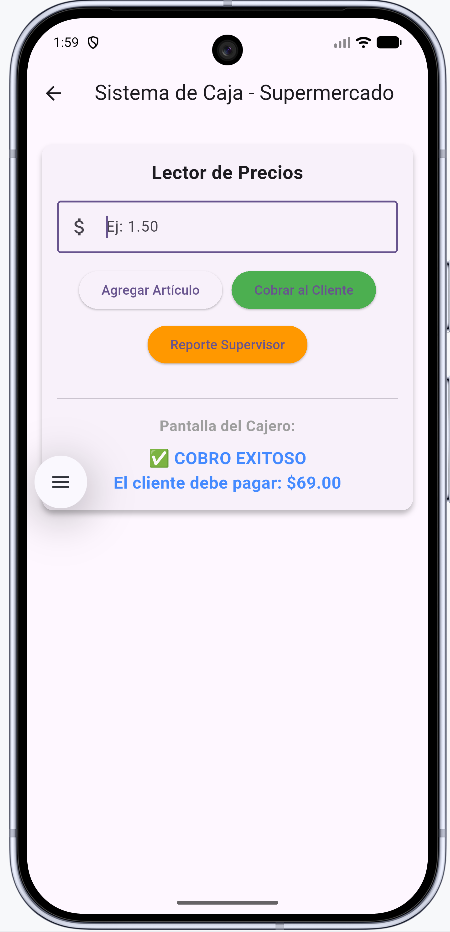
\includegraphics[width=0.4\textwidth]{caja_ejecucion.png}
\end{center}

\newpage
\subsection{Ejercicio 2: Máquina de Vuelto}
\textbf{Problema:} Máquina que da vuelto con monedas de \$2, \$1, \$0.50, \$0.25 y \$0.10. Indicar el vuelto empleando el menor número posible de monedas.

\subsubsection{Pseudocódigo}
\begin{verbatim}
Inicio
  Leer precio, pago
  Si pago < precio Entonces
    Imprimir "Pago insuficiente"
  Sino
    vuelto = pago - precio
    centavos = vuelto * 100
    m2 = centavos DIV 200; centavos = centavos MOD 200
    m1 = centavos DIV 100; centavos = centavos MOD 100
    m50 = centavos DIV 50; centavos = centavos MOD 50
    m25 = centavos DIV 25; centavos = centavos MOD 25
    m10 = centavos DIV 10; centavos = centavos MOD 10
    Imprimir m2, m1, m50, m25, m10
  FinSi
Fin
\end{verbatim}

\subsubsection{Diagrama Nassi-Shneiderman}
\begin{center}
\begin{struktogramm}(130, 70)
  \assign{Leer \texttt{precio}, \texttt{pago}}
  \ifthenelse[15]{1}{1}{\texttt{pago} $<$ \texttt{precio}}{\textbf{Sí}}{\textbf{No}}
    \assign{Imprimir ``Pago Insuficiente''}
  \change
    \assign{\texttt{vuelto} $\gets$ \texttt{pago} - \texttt{precio}}
    \assign{\texttt{cents} $\gets$ \texttt{vuelto} * 100}
    \assign{\texttt{m2} $\gets$ \texttt{cents} DIV 200; \texttt{cents} $\gets$ \texttt{cents} MOD 200}
    \assign{\texttt{m1} $\gets$ \texttt{cents} DIV 100; \texttt{cents} $\gets$ \texttt{cents} MOD 100}
    \assign{\texttt{m50} $\gets$ \texttt{cents} DIV 50; \texttt{cents} $\gets$ \texttt{cents} MOD 50}
    \assign{\texttt{m25} $\gets$ \texttt{cents} DIV 25; \texttt{cents} $\gets$ \texttt{cents} MOD 25}
    \assign{\texttt{m10} $\gets$ \texttt{cents} DIV 10; \texttt{cents} $\gets$ \texttt{cents} MOD 10}
    \assign{Imprimir monedas calculadas}
  \ifend
\end{struktogramm}
\end{center}

\subsubsection{Código (Lógica Central del Modelo)}
\begin{maccode}{lib/model/vuelto\_model.dart}
  static VueltoModelo calcular(double precio, double pago) {
    if (pago < precio) throw Exception("PagoInsuficiente");

    final vuelto = pago - precio;
    int centavos = (vuelto * 100).round();

    final m2 = centavos ~/ 200; centavos %= 200;
    final m1 = centavos ~/ 100; centavos %= 100;
    final m50 = centavos ~/ 50; centavos %= 50;
    final m25 = centavos ~/ 25; centavos %= 25;
    final m10 = centavos ~/ 10; centavos %= 10;

    return VueltoModelo(vueltoTotal: vuelto, monedas2: m2, 
                        monedas1: m1, monedas50: m50, 
                        monedas25: m25, monedas10: m10);
  }
\end{maccode}

\subsubsection{Ejecución}
\begin{center}
    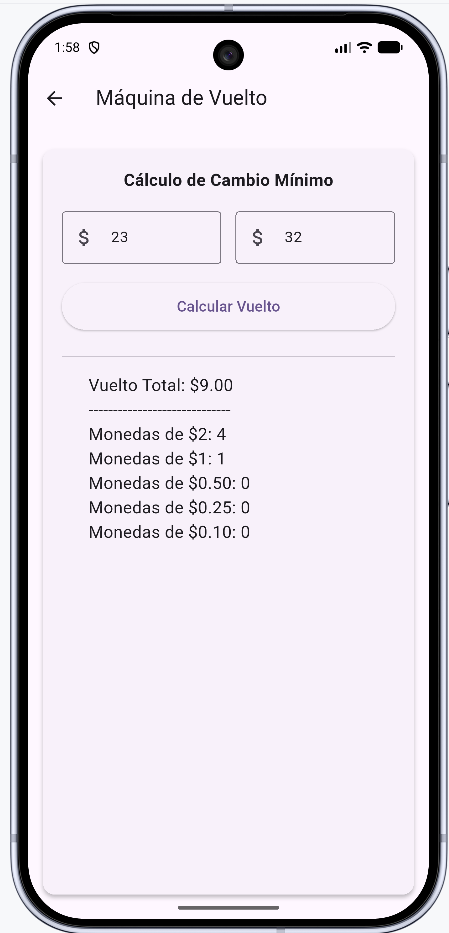
\includegraphics[width=0.4\textwidth]{vuelto_ejecucion.png}
\end{center}


\newpage
\subsection{Ejercicio 3: Año Bisiesto}
\textbf{Problema:} Un año es bisiesto si es múltiplo de 4, exceptuando los múltiplos de 100, que sólo son bisiestos cuando son múltiplos además de 400.

\subsubsection{Pseudocódigo}
\begin{verbatim}
Inicio
  Leer anio
  Si (anio MOD 4 == 0 Y anio MOD 100 != 0) O (anio MOD 400 == 0) Entonces
    esBisiesto = Verdadero
  Sino
    esBisiesto = Falso
  FinSi
  Imprimir esBisiesto
Fin
\end{verbatim}

\subsubsection{Diagrama Nassi-Shneiderman}
\begin{center}
\begin{struktogramm}(130, 40)
  \assign{Leer \texttt{anio}}
  \ifthenelse[15]{1}{1}{(\texttt{anio} \% 4 == 0 $\land$ \texttt{anio} \% 100 $\neq$ 0) $\lor$ (\texttt{anio} \% 400 == 0)}{\textbf{Sí}}{\textbf{No}}
    \assign{\texttt{esBisiesto} $\gets$ Verdadero}
  \change
    \assign{\texttt{esBisiesto} $\gets$ Falso}
  \ifend
  \assign{Imprimir \texttt{esBisiesto}}
\end{struktogramm}
\end{center}

\subsubsection{Código (Lógica Central del Modelo)}
\begin{maccode}{lib/model/bisiesto\_model.dart}
class BisiestoModel {
  bool esBisiesto(int anio) {
    return (anio % 4 == 0 && anio % 100 != 0) || (anio % 400 == 0);
  }
}
\end{maccode}

\subsubsection{Ejecución}
\begin{center}
    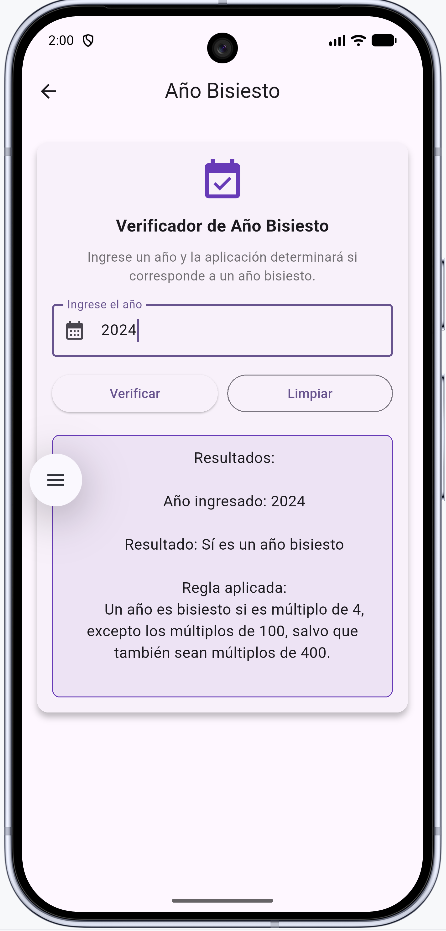
\includegraphics[width=0.4\textwidth]{bisiesto_ejecucion.png}
\end{center}

\newpage
\subsection{Ejercicio 4: Números Perfectos}
\textbf{Problema:} Un número N es perfecto si la suma de sus divisores (excluido el propio N) es N. Hacer un algoritmo que determine si un número es perfecto.

\subsubsection{Pseudocódigo}
\begin{verbatim}
Inicio
  Leer numero
  suma = 0
  Para i desde 1 hasta numero - 1 Hacer
    Si numero MOD i == 0 Entonces
      suma = suma + i
    FinSi
  FinPara
  
  Si suma == numero Entonces
    esPerfecto = Verdadero
  Sino
    esPerfecto = Falso
  FinSi
Fin
\end{verbatim}

\subsubsection{Diagrama Nassi-Shneiderman}
\begin{center}
\begin{struktogramm}(110, 75)
  \assign{Leer \texttt{numero}}
  \assign{\texttt{suma} $\gets$ 0}
  \while{Para \texttt{i} $\gets$ 1 hasta \texttt{numero} - 1}
    \ifthenelse[15]{1}{1}{\texttt{numero} \% \texttt{i} == 0}{\textbf{Sí}}{\textbf{No}}
      \assign{\texttt{suma} $\gets$ \texttt{suma} + \texttt{i}}
    \change
      \assign{Continuar}
    \ifend
  \whileend
  \ifthenelse[15]{1}{1}{\texttt{suma} == \texttt{numero}}{\textbf{Sí}}{\textbf{No}}
    \assign{\texttt{esPerfecto} $\gets$ Verdadero}
  \change
    \assign{\texttt{esPerfecto} $\gets$ Falso}
  \ifend
\end{struktogramm}
\end{center}

\subsubsection{Código (Lógica Central del Modelo)}
\begin{maccode}{lib/model/perfecto\_model.dart}
class PerfectoModel {
  bool esPerfecto(int numero) {
    if (numero <= 1) return false;
    
    int suma = 0;
    for (int i = 1; i < numero; i++) {
      if (numero % i == 0) {
        suma += i;
      }
    }
    return suma == numero;
  }
}
\end{maccode}

\subsubsection{Ejecución}
\begin{center}
    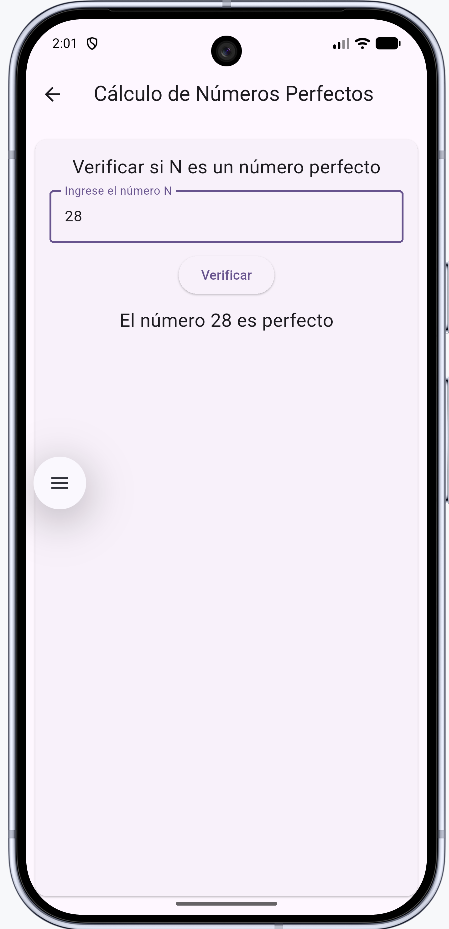
\includegraphics[width=0.4\textwidth]{perfecto_ejecucion.png}
\end{center}

\newpage
\subsection{Ejercicio 5: Control de Peso (Club)}
\textbf{Problema:} Se pesa a cada persona en diez básculas distintas para tener el promedio exacto. Si existe diferencia positiva entre el promedio y el último peso de la última reunión, subieron de peso; si es negativa, bajaron.

\subsubsection{Pseudocódigo}
\begin{verbatim}
Inicio
  Leer pesos[10]
  suma = 0
  Para i desde 1 hasta 10 Hacer
    suma = suma + pesos[i]
  FinPara
  
  promedio = suma / 10
  ultimoPeso = pesos[10]
  diferencia = ultimoPeso - promedio
  
  Si diferencia > 0 Entonces
    estado = "SUBIÓ"
  Sino
    estado = "BAJÓ"
  FinSi
  
  Imprimir promedio, estado, diferencia
Fin
\end{verbatim}

\subsubsection{Diagrama Nassi-Shneiderman}
\begin{center}
\begin{struktogramm}(120, 65)
  \assign{Leer Arreglo \texttt{pesos} de tamaño 10}
  \assign{\texttt{suma} $\gets$ 0}
  \while{Para \texttt{i} $\gets$ 1 hasta 10}
    \assign{\texttt{suma} $\gets$ \texttt{suma} + \texttt{pesos}[i]}
  \whileend
  \assign{\texttt{promedio} $\gets$ \texttt{suma} / 10}
  \assign{\texttt{ultimo} $\gets$ \texttt{pesos}[10]}
  \assign{\texttt{diferencia} $\gets$ \texttt{ultimo} - \texttt{promedio}}
  \ifthenelse[15]{1}{1}{\texttt{diferencia} $>$ 0}{\textbf{Sí}}{\textbf{No}}
    \assign{\texttt{estado} $\gets$ ``SUBIÓ''}
  \change
    \assign{\texttt{estado} $\gets$ ``BAJÓ''}
  \ifend
  \assign{Imprimir \texttt{promedio}, \texttt{estado}}
\end{struktogramm}
\end{center}

\subsubsection{Código (Lógica Central del Modelo)}
\begin{maccode}{lib/model/persona\_modelo.dart}
  static PersonaModelo analizar(List<double> pesos) {
    final suma = pesos.reduce((a, b) => a + b);
    final promedio = suma / pesos.length;
    final ultimo = pesos.last;

    final diferencia = ultimo - promedio;
    final estado = diferencia > 0 ? "SUBIÓ" : "BAJÓ";

    return PersonaModelo(promedio, ultimo, diferencia.abs(), estado);
  }
\end{maccode}

\subsubsection{Ejecución}
\begin{center}
    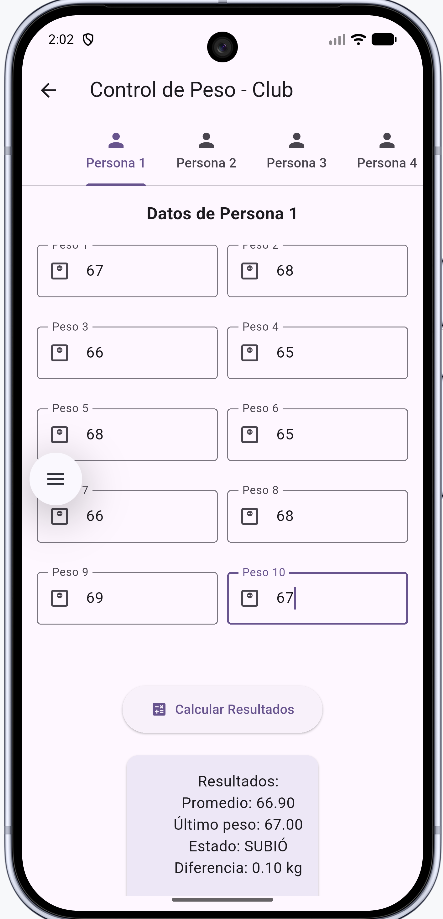
\includegraphics[width=0.4\textwidth]{persona_ejecucion.png}
\end{center}


\newpage
\section{Conclusiones}
\begin{itemize}
    \item La abstracción de algoritmos mediante pseudocódigos y diagramas Nassi-Shneiderman ha permitido diseñar lógicas estructuradas mucho antes de escribir el código fuente, lo que previene errores semánticos y refactorizaciones durante el desarrollo.
    \item La adopción del patrón MVC en el entorno de desarrollo Flutter ha demostrado ser altamente eficiente para separar la lógica de negocio de la gestión de la interfaz de usuario. Extraer la lógica más importante y mostrarla de forma modular ayuda a generar un código más limpio y legible.
    \item En la resolución de problemas (como el cálculo de cambio o la verificación de números perfectos), encapsular la lógica pura dentro del \textit{Modelo} permitió simplificar el código, haciendo que los controladores manejen validaciones de vista y deleguen el comportamiento matemático sin interrupciones.
\end{itemize}

\section{Referencias}
\begin{itemize}
    \item Chapin, N. (1974). \textit{New Format for Flowcharts}. Software: Practice and Experience, 4(4), 341-357.
  \item Google (2024). \textit{Flutter Documentation}. Recuperado de \url{https://docs.flutter.dev/}
  \item Google (2024). \textit{Dart Language Overview}. Recuperado de \url{https://dart.dev/overview}
  \item Google (2024). \textit{Android Studio User Guide}. Recuperado de \url{https://developer.android.com/studio/intro}
    \item Gamma, E., Helm, R., Johnson, R., y Vlissides, J. (1994). \textit{Design Patterns: Elements of Reusable Object-Oriented Software}. Addison-Wesley.
  \item Oracle (2024). \textit{Java Platform, Standard Edition: Java Language Specification}. Recuperado de \url{https://docs.oracle.com/javase/specs/}
\end{itemize}

\section{Anexos}
\subsection{Repositorio de codigo fuente}

\subsubsection{Enlace principal}
\begin{itemize}
  \item \url{https://github.com/LeonelTQL/moviles/tree/main/pry_tarea1}
\end{itemize}

\end{document}
